\section{Related work}

Concepts and vocabulary used here assume previous knowledge of RL and neural
networks. These concepts are more thoroughly described in the background
section, section \ref{sec:background}.

\subsection{Normalized Advantage Functions (NAF)}

In order to extend Q-learning, normally used for discrete state and action
spaces to continuous spaces, Gu et al. \cite{gu2016continuous} proposes a
relatively simple solution called normalized advantage functions (NAF). They
argue after doing simulation experiments that this algorithm is an effective
alternative to recently proposed actor-critic methods and that it learns faster
with more accurate resulting policies. First, the action-value function is
divided into a sum of the value function $V$ and what they call an advantage
function $A : \mathbb{R}^d \longmapsto \mathbb{R}$:

\begin{equation}
    Q(\mathbf{x}, \mathbf{u}) = A(\mathbf{x}, \mathbf{u}) + V(\mathbf{x})
\end{equation}

Here, $\mathbf{x}$ is the state of the environment and $\mathbf{u}$ are
controls or actions. The advantage function is a quadratic function of $u$:

\begin{equation}
    A(\mathbf{x}, \mathbf{u}) = -\frac{1}{2}(\mathbf{u} - \mathbf{\mu(x)})^T\mathbf{P(x)}(\mathbf{u} - \mathbf{\mu(x)})
    \label{eq:advantage_function}
\end{equation}

There are more terms that need to be defined, but first consider equation
(\ref{eq:advantage_function}). The matrix $\mathbf{P}$ is a positive-definite
matrix, this makes the advantage function have its maximum when $\mathbf{u =
\mu(x)}$.  The purpose of $\mu$ is to be a greedy policy function, thus
$\mathbf{Q}$ is maximized when $\mathbf{u}$ is the greedy action. The purpose
of this is that given an optimal $Q$, we do not need to search for the optimal
action, since we know $\mathbf{\mu}$. Now the definition of $\mathbf{P}$:

\begin{equation}
    P(\mathbf{x}) = \mathbf{L(x)L(x)}^T
\end{equation}

Here, $\mathbf{L}$ is a lower-triangular matrix where diagonal entries are
strictly positive.

After these definitions, we are left with estimating the functions $V$,
$\mathbf{\mu}$, and $\mathbf{L}$. To this end the authors use a neural network,
here shown in figure \ref{fig:naf-net}. The $\mathbf{L}$ output is fully
connected with the previous layer and not passed through an activation function
(it is linear). The diagonal entries of L are exponentiated. Hidden layers
consisted of 200 fully connected units with rectified linear units (ReLU) as
activation functions except for $\mathbf{L}$ and $A$ as already defined.

\begin{figure}[h]
    \centering
    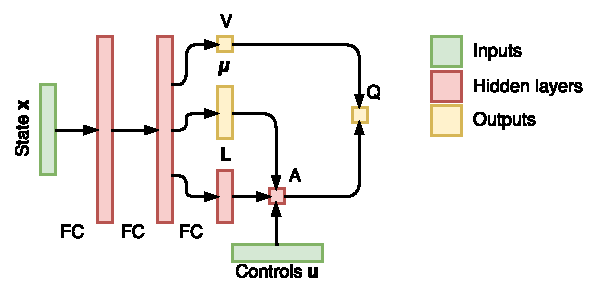
\includegraphics[width=1.0\textwidth]{res/naf-net.pdf}

    \caption{Neural network design for NAF \cite{gu2016continuous}. The
    activation function to $V$ was not specified. The tanh activation was added
    in figure due to Gu et al. \cite{gu2016deep} using it in order to have
    bounded actions for safety reasons.}

    \label{fig:naf-net}
\end{figure}

The NAF algorithm is listed in algorithm \ref{algo:naf}. All collected experiences
are stored in a replay buffer that optimization is run against. Exploration is done
by adding noise to the current greedy policy $\mathbf{\mu}$.

\begin{algorithm}[!h]
    \caption{NAF algorithm}
    \begin{algorithmic}
        \STATE{Randomly initialize network $Q(x, u|\theta)$}
        \STATE{Initialize target network $Q'$, $\theta' \leftarrow \theta$}
        \STATE{Initialize replay buffer $R \leftarrow \emptyset$}
        \FOR{episode $= 1$ to $M$}
            \STATE{Initialize random process $\mathcal{N}$ for action exploration}
            \STATE{Receive initial exploration state $x_1$}
            \FOR{$t = 1$ to $T$}
                \STATE{Select action $\mathbf{u_t = \mu(x_t|\theta) + \mathcal{N}_t}$}
                \STATE{Execute $\mathbf{u_t}$ and observe $r_t$ and $\mathbf{x}_{t+1}$}
                \STATE{Store transition $(\mathbf{x}_t, \mathbf{u}_t, r_t, \mathbf{x}_{t+1})$ in $R$}
                \FOR{iteration $= 1$ to $I$}
                    \STATE{Sample a random minibatch of $m$ transitions from $R$}
                    \STATE{Set $y_i = r_i + \gamma V'(\mathbf{x}_{i+1}|\theta')$}
                    \STATE{Update $\theta$ by minimizing the loss:
                           $L = \frac{1}{N}\sum_i (y_i - Q(\mathbf{x}_i, \mathbf{u}_i|\theta))^2$}
                    \STATE{Update target network $\theta' \leftarrow \tau \theta + (1 - \tau)\theta'$}
                \ENDFOR
            \ENDFOR
        \ENDFOR
    \end{algorithmic}
    \label{algo:naf}
\end{algorithm}

\subsection{Distributed real-world learning using NAF}
\label{sec:distributed_naf}

Real-world experiments were done by Gu et al. \cite{gu2016deep} on door opening
tasks using the NAF algorithm and 7-DoF torque controlled arms. They extended
the algorithm to be distributed on several robots/collectors and one separate
trainer thread on a separate machine. They state that this was the first
successful real-world experiment with a relatively high complexity problem
without human demonstration or simulated pretraining. They used the layout of
the network shown in figure \ref{fig:naf-net} but with hidden layers of 100
units each. Also, in this article it was explicitly mentioned that the
activation functions for the policy $\mathbf{\mu}$ was tanh in order to bound
the actions. The state input consisted of the arm pose and target pose. The
target pose was known from attached equipment. The modified version of NAF is
listed in algorithm \ref{algo:async_naf}.

The authors conclude that there was an upper bound on the effects of
parallelization, but hypothesize that the speed of the trainer thread has a
limiting factor in this matter. They used CPU for training the neural network
so instead using a GPU might increase the effect of more collectors.

\begin{algorithm}[!h]
    \caption{Asynchronous NAF - $N$ collector threads and $1$ trainer thread}
    \begin{algorithmic}
        \STATE{// trainer thread}
        \STATE{Randomly initialize network $Q(\mathbf{x}, \mathbf{u}|\theta)$}
        \STATE{Initialize target network $Q'$, $\theta' \leftarrow \theta$}
        \STATE{Initialize shared replay buffer $R \leftarrow \emptyset$}
        \FOR{iteration $= 1$ to $I$}
            \STATE{Sample a random minibatch of m transitions from $R$}
            \STATE{Set $y_i = \begin{cases}r_i+\gamma V'(x_i|\theta) &\text{ if } t_i < T,\\r_i &\text{ if } t_i = T\end{cases}$}
            \STATE{Update $\theta$ by minimizing the loss:
                   $L = \frac{1}{m} \sum_i (y_i - Q(\mathbf{x}_i, \mathbf{u}_i|\theta))^2$}
            \STATE{Update the target network: $\theta' \leftarrow \tau\theta + (1-\tau)\theta'$}
        \ENDFOR
        \STATE{// collector thread $n$, $n = 1...N$}
        \FOR{episode $= 1$ to $M$}
            \STATE{Sync policy network weights $\theta_n \leftarrow \theta$}
            \STATE{Initialize a random process $\mathcal{N}$ for action exploration}
            \STATE{Receive initial observation state $x_1$}
            \FOR{$t = 1$ to $T$}
                \STATE{Select action $\mathbf{u}_t = \mathbf{mu}$}
                \STATE{Execute $\mathbf{u}_t$ and observe $r_t$ and $\mathbf{x}_{t+1}$}
                \STATE{Send transition $(\mathbf{x}_t, \mathbf{u}_t, r_t, \mathbf{x}_{t+1}, t)$ to $R$}
            \ENDFOR
        \ENDFOR
    \end{algorithmic}
    \label{algo:async_naf}
\end{algorithm}

\subsection{Spatial softmax in pose estimation}

Levine et al. \cite{levine2016end} proposed an architecture for a CNN that
gives pose estimates for robotic manipulation tasks. After the last
convolutional layer, a softmax is applied, but only normalized over each
kernel's response map, called \textit{spatial softmax}:

\begin{equation}
    s_{cij} = \frac{e^{a_{cij}}}{\sum_{i',j'} e^{a_{ci'j'}}}
\end{equation}

Here, $a_{cij}$ is the output of the $c$:th kernel at coordinate $ij$. After
this, they calculate the expected 2D position for each feature, which they
argue is better suited for pose estimation. The expected 2D position is
expressed as a tuple $(f_{cx}, f_{cy})$ calculated according to:

\begin{align}
    f_{cx} &= \sum_{i,j} s_{ij} x_{ij} \\
    f_{cy} &= \sum_{i,j} s_{ij} y_{ij}
\end{align}

The scalar value $x_{ij}$ is the position in image space of the pixel at coordinate
$(i, j)$. This can reasonably easy be simplified to a matrix multiplication with constant
weights from each of the response maps. Arguably, it could also be possible to rewrite the
above expressions as:

\begin{align}
    f_{cx} &= \sum_{i,j} i s_{ij} \\
    f_{cy} &= \sum_{i,j} j s_{ij}
\end{align}

\subsection{Door opening with human demonstration}

Chebotar et al. \cite{chebotar2016path} demonstrates door opening tasks
initialized from human demonstration using methods called Guided Policy Search
(GPS) and Policy Improvement with Path Integrals (PI$^2$). They demonstrate
that they can learn this task outputting torque control from visual input. This is
extended by Yahya et al. \cite{yahya2016collective} to be trained
simultaneously on several robots. In both cases, torque commands are the output
of a neural network where the first part takes visual input and is pretrained
with pose estimates of the door and the robot arm. This neural network is shown
in figure \ref{fig:gps_net}. Since the robot poses were labeled in the robot
base frame and the camera offsets were somewhat random, a linear mapping from
the neural network output to the base frame was learned separately for each of
the robots. The authors evaluated the trained policy on a previously unseen
door with different translations and rotations. The mean success rate was
90\%. They also tried offsetting the camera 1) 5 cm towards the ground and 2) 4
cm backwards. The respective success rates for these translations were 52 \%
and 54 \%.

\begin{figure}[h]
    \centering
    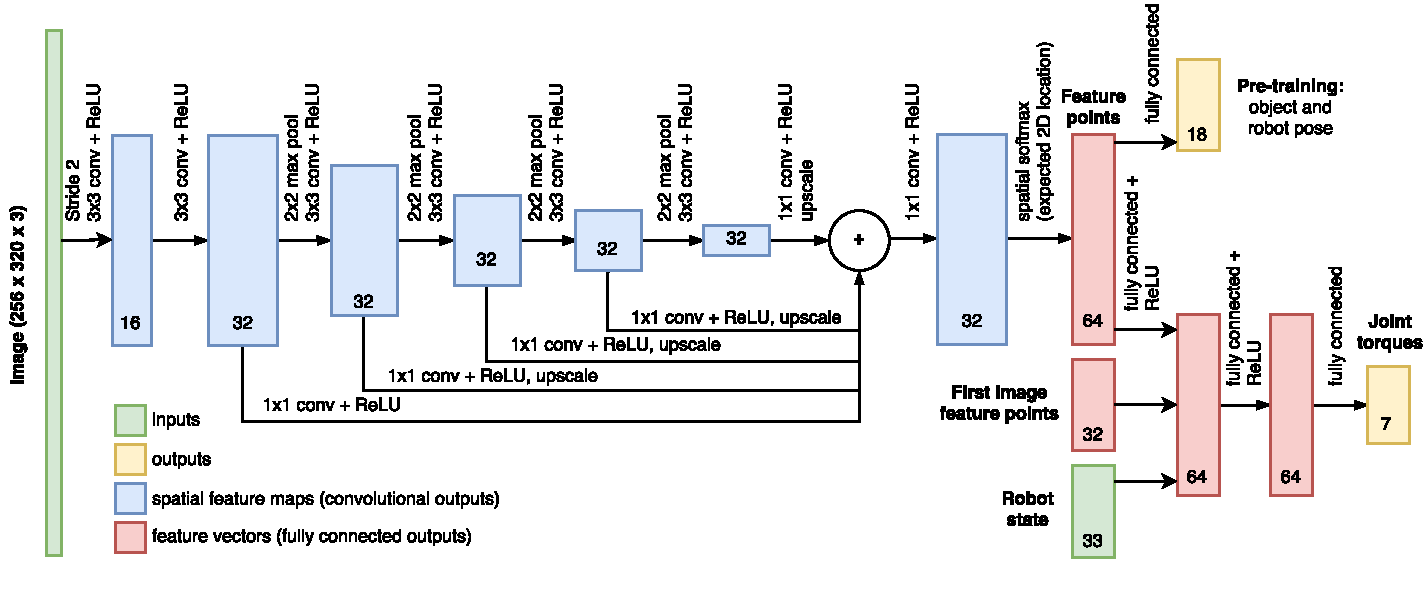
\includegraphics[width = 1.0\textwidth]{res/gps-net.pdf}
    \caption{Network used for door opening task from visual inputs \cite{chebotar2016path}}
    \label{fig:gps_net}
\end{figure}

\subsection{Prioritized experience replay}
\label{sec:prio_sampling}

When randomly sampling experiences from a replay buffer, one alternative is to
sample from a uniform distribution. However, if samples are sampled from a
distribution where experiences with larger temporal-difference errors are more
likely to be chosen, training times can be reduced with resulting policies that
outperform those trained by uniform sampling \cite{schaul2015prioritized}. Let
$R_{t}$ be the reward at time $t$, $Q(S_t, A_t)$ the Q-function of state $S_t$
and action $A_t$ at time $t$ and $V(S_t)$ the value function for $S_t$ at time
$t$. Given a sample tuple $x_i = (S_t, S_{t+1}, A_t, R_{t+1})$, let the
temporal-difference error for this sample to be defined as:

\begin{equation}
    \delta_i = Q(S_{t}, A_t) - \left[ R_{t+1} + V(S_{t+1}) \right]
\end{equation}

Define a priority $p_i$ of sample $x_i$ as:

\begin{equation}
    p_i = |\delta_i| + \epsilon
\end{equation}

Here $\epsilon > 0$ ensures all priorities are strictly positive. Sample experiences
according to the probability:

\begin{equation}
    P(i) = \frac{p_i^\alpha}{\sum_k p_k^\alpha}
\end{equation}

The hyperparameter $\alpha \geq 0$ enforces more uniform probabilities for values close to
zero and more non-uniform probabilities for larger values.

Since the gradient is biased by a biased choice of samples, the magnitude of
the gradient with respect to each sample $x_i$ can be weighted by:

\begin{equation}
    w_i = \left( \frac{1}{P(i)} \right)^\beta
\end{equation}

The parameter $\beta \geq 0$ can be varied during training, and it is argued that
the unbiased gradient are more important towards the end when the policy is
converging. They varied this parameter reaching $\beta = 1$ only towards the
end of the training. It is not clear from the article but it is assumed that
training starts with $\beta = 0$.

%\subsection{Motion planning by a predictive model}
%
%Another method for learning manipulation tasks was shown by Finn and Levine
%\cite{finn2016deep}. Given a sequence of initial images, they denote it
%$I_{0:1}$, together with robot poses $x_{0:1}$, and future commands $a_{1:H_p}$
%where $H_p$ is some prediction horizon, they predict the distribution of future
%images $I_{2:H_p + 1}$. $I_t$ is here a collection of independent pixel
%distributions with mean $\hat{I}_t$. A convolutional LSTM was used for this,
%and an implicit feature of the network is what they call a flow map
%$\hat{F}_t(x, y, k, l)$ which is the probability of the pixel at coordinates
%$(k, l)$ at time $t+1$ originating from coordinates $(x, y)$. Given a flow map
%they can do one step prediction:
%
%\begin{equation}
%    \hat{F}_t \odot \hat{I}_t := \sum_{k \in (-\kappa, \kappa)} \sum_{l \in (-\kappa, \kappa)} \hat{F}_t(x,y,k,l)\hat{I}_t(x-k, y-l) = \hat{I}_{t+1}
%\end{equation}
%
%When using these implicit flow operators rather than actual predicted image
%which was the output from the network, they can predict movement of individual
%pixels for several time steps ahead. Using a maximum likelihood approach, they
%can find the series of actions that puts a pixel at some other target location.
%For evaluation, they try their trained algorithm on previously unseen objects
%by selecting start and end coordinates for which it generalized.
%
%An interesting feature of their approach is that the data set for training was
%generated by torque-controlled arms randomly interacting with a collection of
%objects and recording images of it along with the robot poses. Therefore, no
%part of the training needed human supervision or demonstration. Another feature
%is that the camera positions were not the same across robots, it is unclear if
%they evaluated the method with a new camera position though.
%
